\section{Differentiation}
\subsection{Defining the Derivative}
Given a function $f: U \subseteq \R \rightarrow \R$. The \textbf{derivative} of $f$ is,
\[
\deriv(x) =\lim _{h \rightarrow 0} \frac{f(x+h)-f(x)}{h}
\]

\noindent We want to generalize this to functions of more than one variable.

\begin{defn}[Partial Derivative]
    \sloppy Let $U \subseteq \R^n$ be an open set. Given a function $f: U \subseteq \R^n \rightarrow \R$, the \textbf{partial derivative} of $f$ is,
    \[\frac{\partial f}{\partial x_j}(x_1, \cdots, x_n) =\lim _{h \rightarrow 0} \frac{f\left(x_1, \ldots, x_j+h, \ldots, x_n\right)-f\left(x_1, \ldots, x_n\right)}{h}\]
\end{defn}

\begin{rmk}
If the partial derivative of a function, e.g., $f: \R^2 \rightarrow \R$, is being evaluated at a point, e.g., $\mathbf{x}_0 = (x_0, y_0) \in \R^2$, we write,
\[
f_x(x_0, y_0) \quad \text{ or } \quad
\frac{\partial f}{\partial x}\left(x_0, y_0\right) \quad \text { or }\left.\quad \frac{\partial f}{\partial x}\right|_{\mathbf{x}_0} \quad\]
\end{rmk}

\begin{marginfigure}
    The graph of $f: \R^2 \rightarrow \R$ defined by,
        \[f(x, y) = x^{1/3} \cdot y^{1/3}\]
    does not have a tangent plane at $(0,0)$,
    \begin{center}
       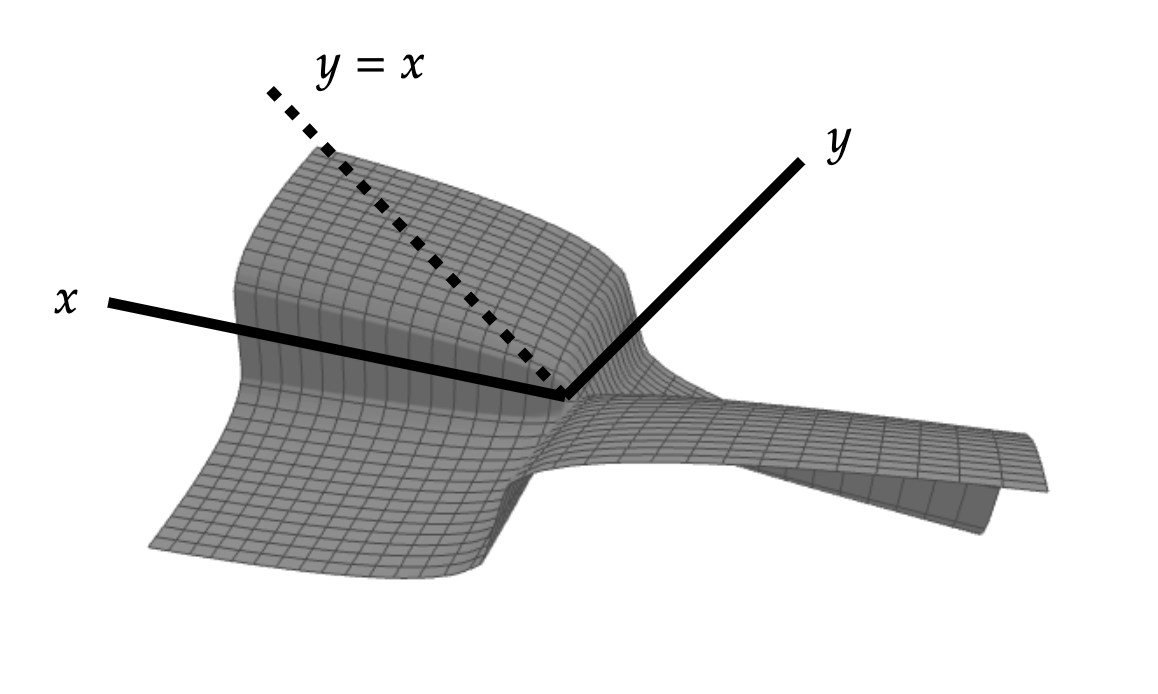
\includegraphics[width=\textwidth]{figures/wk-2/case-study.png}
    \end{center}
    Its contour plot is shown below, 
    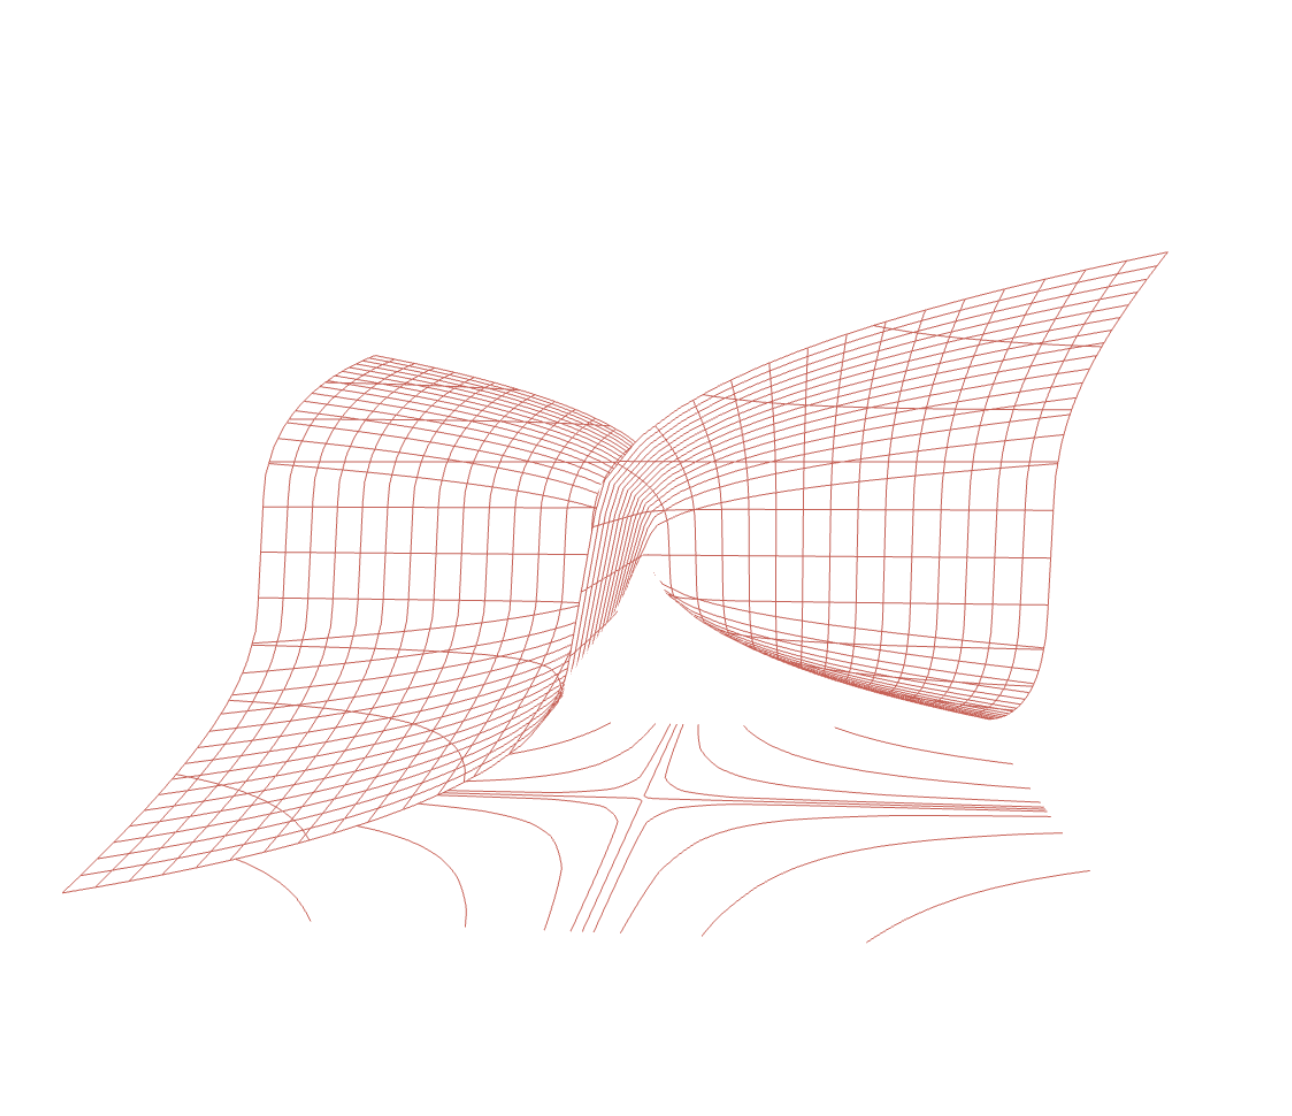
\includegraphics[width=0.8\linewidth]{figures/wk-2/fig-23.png}
\end{marginfigure}

\begin{ex}{Existence of the Partial Derivatives}{label}
    Let $f(x, y) = x^{1/3} \cdot y^{1/3}$. By definition,
    \begin{align*}
        &f_x(0,0)=\lim_{h \rightarrow 0} \frac{f(h, 0)-f(0,0)}{h}=\lim_{h \rightarrow 0} \frac{0-0}{h}=0 \\
        &f_y(0,0)=\lim_{h \rightarrow 0} \frac{f(0, h)-f(0,0)}{h}=\lim_{h \rightarrow 0} \frac{0-0}{h}=0
    \end{align*}
    Thus, $f_y(0,0) = f_x(0,0) = 0$. Consider the restriction of $f(x, y)$ to the line $y = x$. We obtain $f(x, x) = x^{2/3}$, which we know from one-variable calculus is not differentiable at $(0,0)$.
\end{ex}

\begin{ex}{Computing Partial Derivatives}{label}
Let $f: \R^2 \rightarrow \R$ be defined by $f(x, y) = e^{x^2 y}$. We compute,
\[\frac{\partial f}{\partial x} = e^{x^2 y} \cdot 2xy \quad \text{ and } \quad \frac{\partial f}{\partial y} = e^{x^2 y} \cdot x^2\]
\end{ex}

\begin{defn}[Linear Approximation]
    \sloppy The \textbf{linear approximation} $L f |_{\mathbf{x}_0}$ to $\texttt{graph}(f)$ at the point $\mathbf{x}_0 = (x_0, y_0)$ is given by,
    \[
    z = f\left(x_0, y_0\right)+\left[\frac{\partial f}{\partial x}\left(x_0, y_0\right)\right]\left(x-x_0\right)+\left[\frac{\partial f}{\partial y}\left(x_0, y_0\right)\right]\left(y-y_0\right)
    \]
\end{defn}

\begin{defn}[Differentiability]
    A function $f: \R^2 \rightarrow \R$ is \textbf{differentiable} at $\mathbf{x}_0$ if the partial derivatives $f_x$ and $f_y$ exist and we have that,
    \[\lim_{\mathbf{x} \rightarrow \mathbf{x}_0} \frac{f(\mathbf{x}) - L f |_{\mathbf{x}_0}}{\|\mathbf{x} - \mathbf{x}_0\|} = 0\]
\end{defn}

\begin{cor}
    If $f$ is differentiable at $\mathbf{x}_0$, then $L f |_{\mathbf{x}_0}$ is called the \textbf{tangent plane} of $\texttt{graph}(f)$ at the point $(x_0, y_0, f(x_0, y_0)) \in \R^3$.
\end{cor}

\begin{ex}{Finding the Equation of the Tangent Plane}{label}
    Consider the function $f: \R^2 \rightarrow \R$ defined by,
    \[f(x, y)=1-x^2-y^2\]
    The equation of the tangent plane at,
    \[\left(x_0, y_0\right)=(1 / \sqrt{3}, 1 / \sqrt{3})\]
    is given by,
    \[z-1 / 3=-\frac{2}{\sqrt{3}}\left(x-\frac{1}{\sqrt{3}}\right)-\frac{2}{\sqrt{3}}\left(y-\frac{1}{\sqrt{3}}\right)\]
\end{ex}

\begin{marginfigure}
\begin{center}
       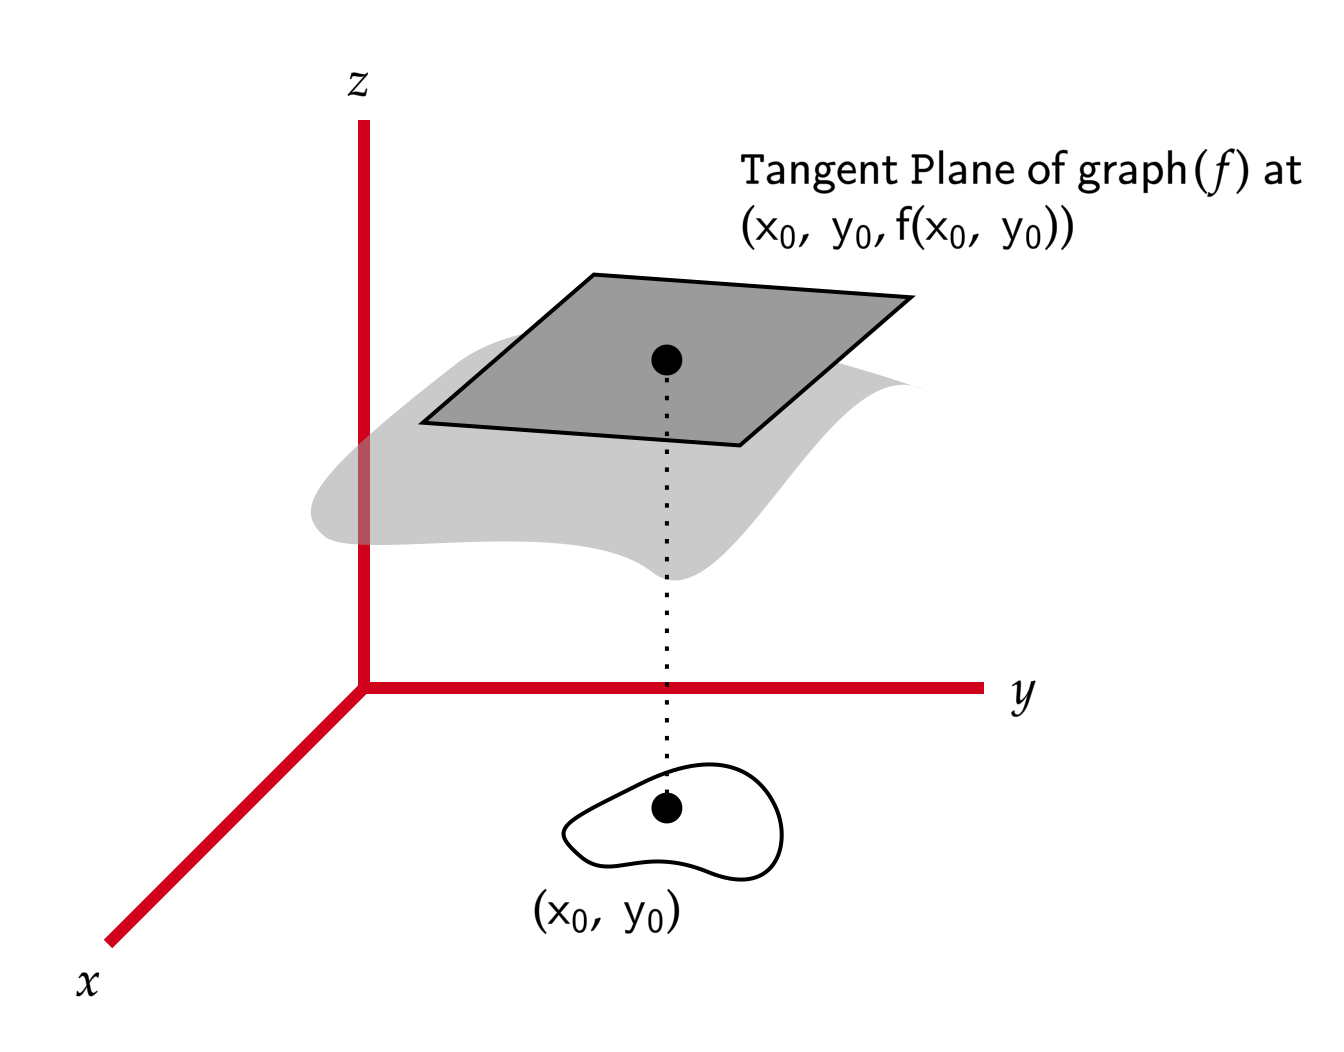
\includegraphics[width=\textwidth]{figures/wk-2/fig-25.png}
\end{center}
\end{marginfigure}

\begin{defn}[Jacobian]
    Let $U \subseteq \R^n$ be an open set. Given a function $f: U \subseteq \R^n \rightarrow \R^m$, the \textbf{derivative} $(\mathbf{D} f)(\mathbf{x})$ is,
    \[
    (\mathbf{D} f)(\mathbf{x})=\left[\begin{array}{ccc}
    \frac{\partial f_1}{\partial x_1} & \cdots & \frac{\partial f_1}{\partial x_n} \\
    \vdots & & \vdots \\
    \frac{\partial f_m}{\partial x_1} & \cdots & \frac{\partial f_m}{\partial x_n}
    \end{array}\right]
    \]
    which we call the \textbf{Jacobian matrix}.
\end{defn}

\begin{rmk}
The Jacobian matrix can be thought of as a linear map from $\R^n$ to $\R^m$. When $m = 1$, the \textbf{gradient} $\nabla f$ is the $1 \times n$ matrix,
\[
    \nabla f := (\mathbf{D} f) =\left[\begin{array}{lll}
    \frac{\partial f}{\partial x_1} & \cdots & \frac{\partial f}{\partial x_n}
    \end{array}\right]
\]
\end{rmk}

\begin{defn}
    Let $U \subseteq \R^n$ be an open set. A function $f: U \subseteq \R^n \rightarrow \R^m$ is \textbf{differentiable} at $\mathbf{x}_0$ if the partial derivatives exist at $\mathbf{x}_0$ and,
    \[\lim_{\mathbf{x} \rightarrow \mathbf{x}_0} \frac{\|f(\mathbf{x}) - (L f |_{\mathbf{x}_0})\|}{\|\mathbf{x} - \mathbf{x}_0\|} = 0\]
    where,
    \[L f |_{\mathbf{x}_0} = \underbrace{f(\mathbf{x}_0)}_{\in \R^m} + \underbrace{(\mathbf{D} f)(\mathbf{x}_0)}_{\R^n \rightarrow \R^m} \cdot \underbrace{(\mathbf{x} - \mathbf{x}_0)}_{\in \R^m}\]
\end{defn}

\begin{marginfigure}
    The graph of $f: \R^2 \rightarrow \R$ defined by,
    \[f(x,y) := \begin{cases}
         \frac{xy}{x^2 + y^2} & \text{ for } (x, y) \neq (0,0) \\
         0 & \text{otherwise}
      \end{cases}
    \]
    \begin{center}
        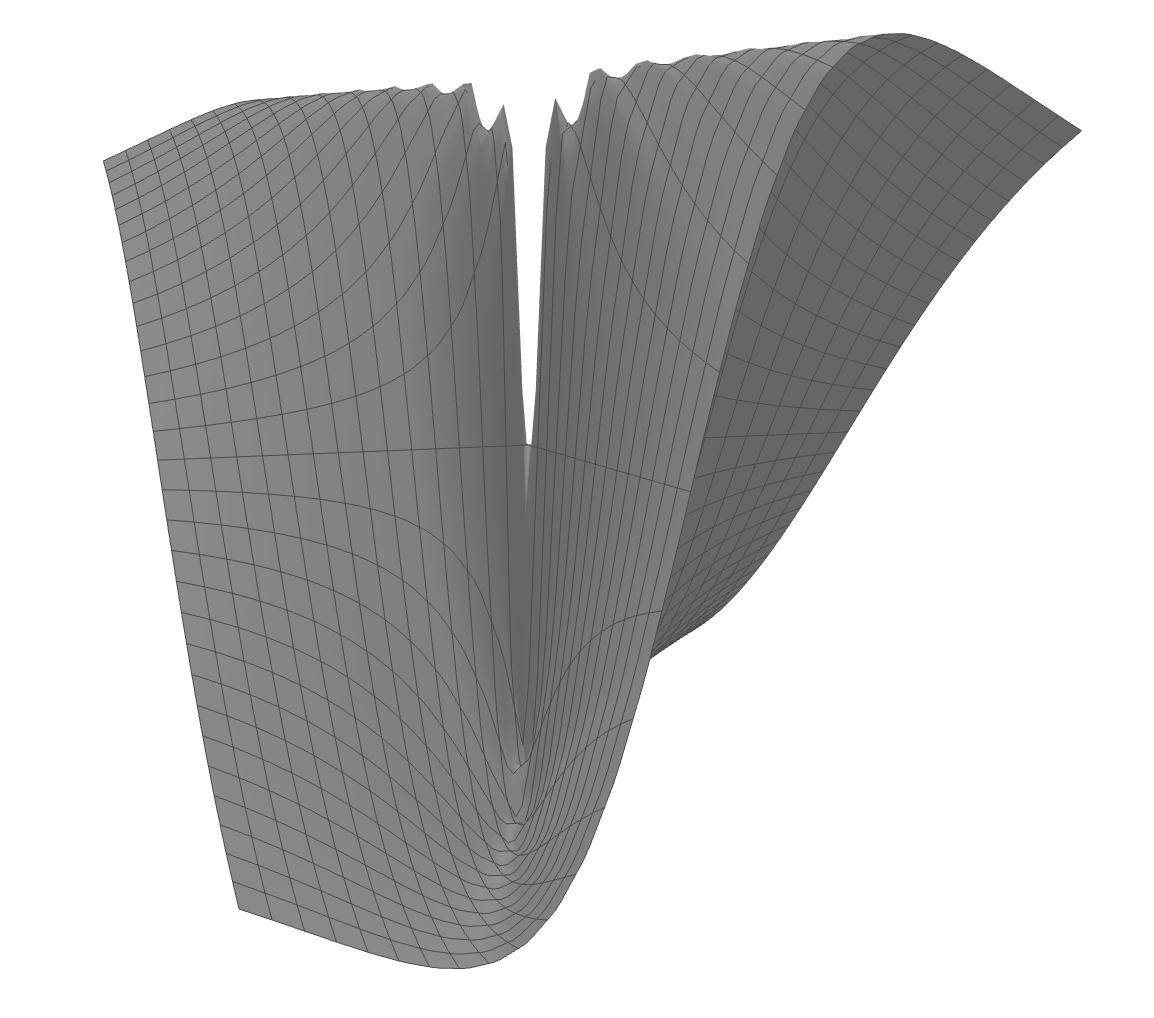
\includegraphics[width=0.6\linewidth]{figures/wk-2/fig-22.png}
    \end{center}
    Its contour plot is shown below,
    \begin{center}
        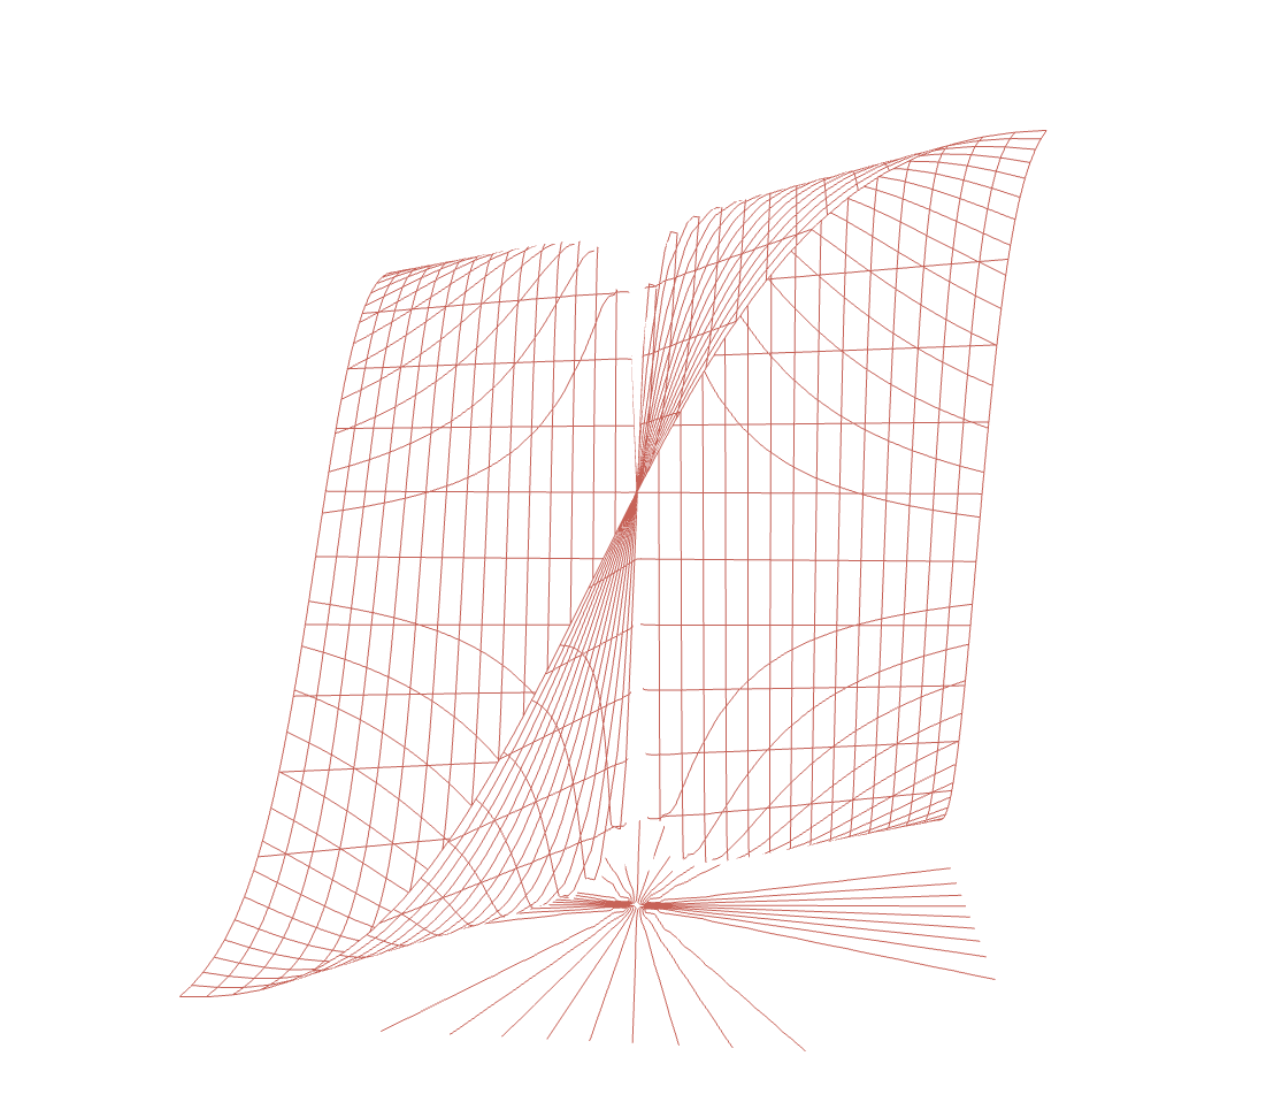
\includegraphics[width=0.8\linewidth]{figures/wk-2/fig-21.png}
    \end{center}
\end{marginfigure}

\begin{thm}
    Let $f: U \subseteq \R^n \rightarrow \R^m$. Then,
    \begin{enumerate}
        \item If $f$ is differentiable at $\mathbf{x}_0$, then $f$ is continuous at $\mathbf{x}_0$
        \item \sloppy If the partial derivatives $\partial f_i / \partial x_j$ exist and are continuous in a neighborhood of $\mathbf{x}_0$, then $f$ is differentiable at $\mathbf{x}_0$
    \end{enumerate}
\end{thm}

\begin{ex}{Continuity of the Partial Derivatives}{label}
    The existence of the partial derivatives does not guarantee continuity. Consider the function $f: \R^2 \rightarrow \R$ defined by,
    \[
    f(x,y) := \begin{cases}
         \frac{xy}{x^2 + y^2} & \text{ for } (x, y) \neq (0,0) \\
         0 & \text{otherwise}
         \end{cases}
    \]
    The partial derivatives of $f$ exist,
    \begin{align*}
        &f_x(0,0)=\lim _{h \rightarrow 0} \frac{f(h, 0)-f(0,0)}{h}=\lim _{h \rightarrow 0} \frac{\frac{0}{h^2}-0}{h}=0 \\
        &f_y(0,0)=\lim _{h \rightarrow 0} \frac{f(0, h)-f(0,0)}{h}=\lim _{h \rightarrow 0} \frac{\frac{0}{h^2}-0}{h}=0
    \end{align*}
    but $f$ is not continuous at the origin,
    \[\lim _{x \rightarrow 0} f(x, x)=\frac{1}{2} \neq f(0,0)\]
    \texttt{graph}$(f)$ is shown in the margin.
\end{ex}

\subsection{Sums, Products, and Quotients}
\begin{thm}[Sums, Products, and Quotients]
    Let $f: U \subset \mathbb{R}^n \rightarrow \mathbb{R}^m$ and $g: U \subset \mathbb{R}^n \rightarrow \mathbb{R}^m$ be differentiable at $\mathbf{x}_0 \in U$.
    \begin{enumerate}
        \item \textbf{(Constant Rule)} Let $c \in \R$. $c f(x)$ is differentiable at $\mathbf{x}_0$, and,
        \[(\mathbf{D} c f)\left(\mathbf{x}_0\right)=c (\mathbf{D} f)\left(\mathbf{x}_0\right)\]
        \item \textbf{(Sum Rule)} $f(x) + g(x)$ is differentiable at $\mathbf{x}_0$, and,
        \[(\mathbf{D} (f + g))\left(\mathbf{x}_0\right)=(\mathbf{D} f)\left(\mathbf{x}_0\right)+(\mathbf{D} g)\left(\mathbf{x}_0\right)\]
    \end{enumerate}
    The following two properties hold when $m = 1$,
    \begin{enumerate}
        \item \textbf{(Product Rule)} $g(x) f(x)$ is differentiable at $\mathbf{x}_0$, and,
        \[\mathbf{D}(g f)(\mathbf{x}_0) = g(\mathbf{x}_0)(\mathbf{D}f)(\mathbf{x}_0) + f(\mathbf{x}_0)(\mathbf{D} g)(\mathbf{x}_0)\]
        \item \textbf{(Quotient Rule)} $f(x)/g(x)$ is differentiable at $\mathbf{x}_0$, and,
        \[\mathbf{D}(f / g)(\mathbf{x}_0) = \frac{g(\mathbf{x}_0)(\mathbf{D}f)(\mathbf{x}_0) + f(\mathbf{x}_0)(\mathbf{D} g)(\mathbf{x}_0)}{(g(\mathbf{x}_0))^2} \quad \text{ and } \quad g(\mathbf{x}_0) \neq 0\]
    \end{enumerate}
\end{thm}

\subsection{Chain Rule}
\begin{thm}[Chain Rule]
    Let $g: U \subset \mathbb{R}^n \rightarrow \mathbb{R}^m$ and $f: U \subset \mathbb{R}^m \rightarrow \mathbb{R}^p$. If $g$ is differentiable at $\mathbf{x}_0$ and $f$ is differentiable at $g(\mathbf{x}_0)$, then,
    \[\mathbf{D}(f \circ g)\left(\mathbf{x}_0\right)=(\mathbf{D} f)\left(\mathbf{y}_0\right) (\mathbf{D} g) \left(\mathbf{x}_0\right)\]
\end{thm}

\begin{marginfigure}
\begin{center}
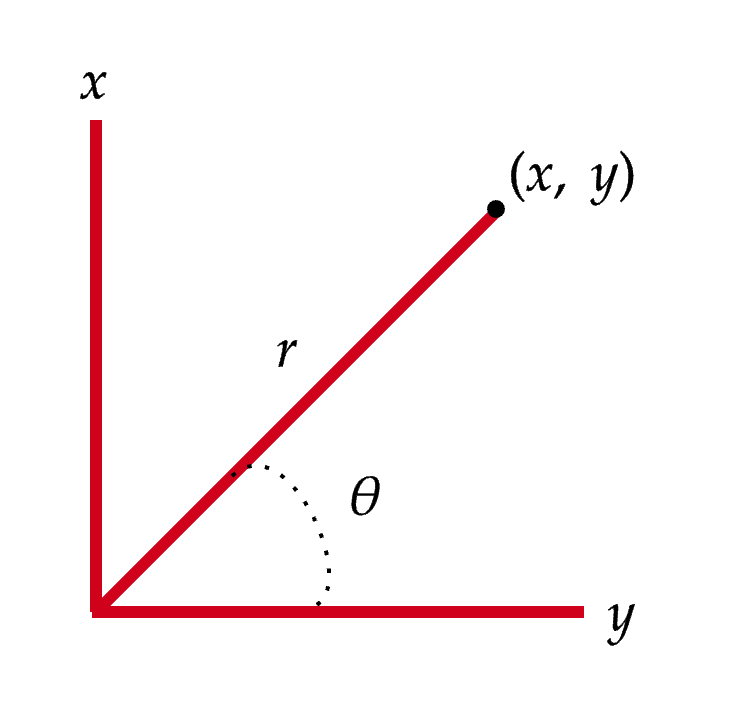
\includegraphics[width=0.8\textwidth]{figures/wk-2/fig-26.png}
\end{center}
\end{marginfigure}

\begin{ex}{Polar Coordinates}{label}
    We can relate a set of \textbf{polar coordinates} $(r, \theta)$ to each point \text{$(x, y) \in \R^2$} expressed in \textbf{Cartesian coordinates}. Observe,
    \[x=r \cos \theta \quad \text{ and } \quad y=r \sin \theta\]
    where $r \geq 0$ and $0 \leq \theta < 2\pi$.
    Consider the composition,
    \[(r, \theta) \stackrel{f}{\longmapsto}(x = r \cos \theta, y = r \sin \theta) \stackrel{g}{\longrightarrow} g(x, y)\]
    Fix a point $\mathbf{x}_0 = (r, \theta)$. We will compute $(\mathbf{D}g)(\mathbf{x}_0)$:
    \[(\mathbf{D}f)(\mathbf{x}_0)=\left(\begin{array}{cc}\frac{\partial f_1}{\partial r} & \frac{\partial f_1}{\partial \theta} \\ \frac{\partial f_2}{\partial r} & \frac{\partial f_2}{\partial \theta}\end{array}\right)=\left(\begin{array}{cc}\cos \theta & -r \sin \theta \\ \sin \theta & r \cos \theta\end{array}\right)\]
    \[
    (\mathbf{D} g)\left(f\left(\mathbf{x}_0\right)\right)=\left(\begin{array}{ll}\frac{\partial g}{\partial x} & \frac{\partial g}{\partial y}\end{array}\right)(x=r \cos \theta, y=r \sin \theta)
    \]
    Therefore, 
    \begin{align*}
    \mathbf{D}(g \circ f)&=
    \left(\begin{array}{ll}\frac{\partial g}{\partial x} & \frac{\partial g}{\partial y}\end{array}\right)\left(\begin{array}{cc}\cos \theta & -r \sin \theta \\ \sin \theta & r \cos \theta\end{array}\right) \\
    &=\left(\frac{\partial g}{\partial x} \cos \theta+\frac{\partial g}{\partial y} \sin \theta-\frac{\partial g}{\partial x} r \sin \theta+\frac{\partial g}{\partial y} r \cos \theta\right)
    \end{align*}
    by the Chain Rule.
\end{ex}

\begin{ex}{Simple Function Composition}{label}
    Consider $f: \R \rightarrow \R^2$ and $g: \R^2 \rightarrow \R$ defined by,
    \begin{align*}
        &f(t) = (t, t^2) \\
        &g(x, y) = x^2 + y^2
    \end{align*}
    We begin by computing the partial derivatives of $f$ and $g$,
    \[\nabla g=(2 x \quad 2 y) \quad \text{ and } \quad \nabla f=\left(\begin{array}{l}
        1 \\
        2 t
        \end{array}\right)\]

    We can compute $(\mathbf{D} g \circ f)(t)$ as follows,
    \begin{align*}
        (\mathbf{D} g \circ f)(t)&=(\mathbf{D} g)(f(t)) \cdot(\mathbf{D} f)(t) \\
        &=\left(2 t, 2 t^2\right) \cdot\left(\begin{array}{l}
            1 \\
            2 t
            \end{array}\right) \\
        &=2 t+2 t \\
        &=4 t
    \end{align*}
    since $(\mathbf{D} g)(f(t))=\left(2 t, 2 t^2\right)$.
\end{ex}

\subsection{Paths and Curves}
\begin{defn}[Curve]
    \sloppy A \textbf{curve} is the image of a set of real numbers, called a \textbf{path}. We write $t$ for the independent variable, so that $\mathbf{c}(t)$ is its position. The path \textbf{c} is said to \textbf{parameterize} the curve.
\end{defn}

\begin{marginfigure}
\begin{center}
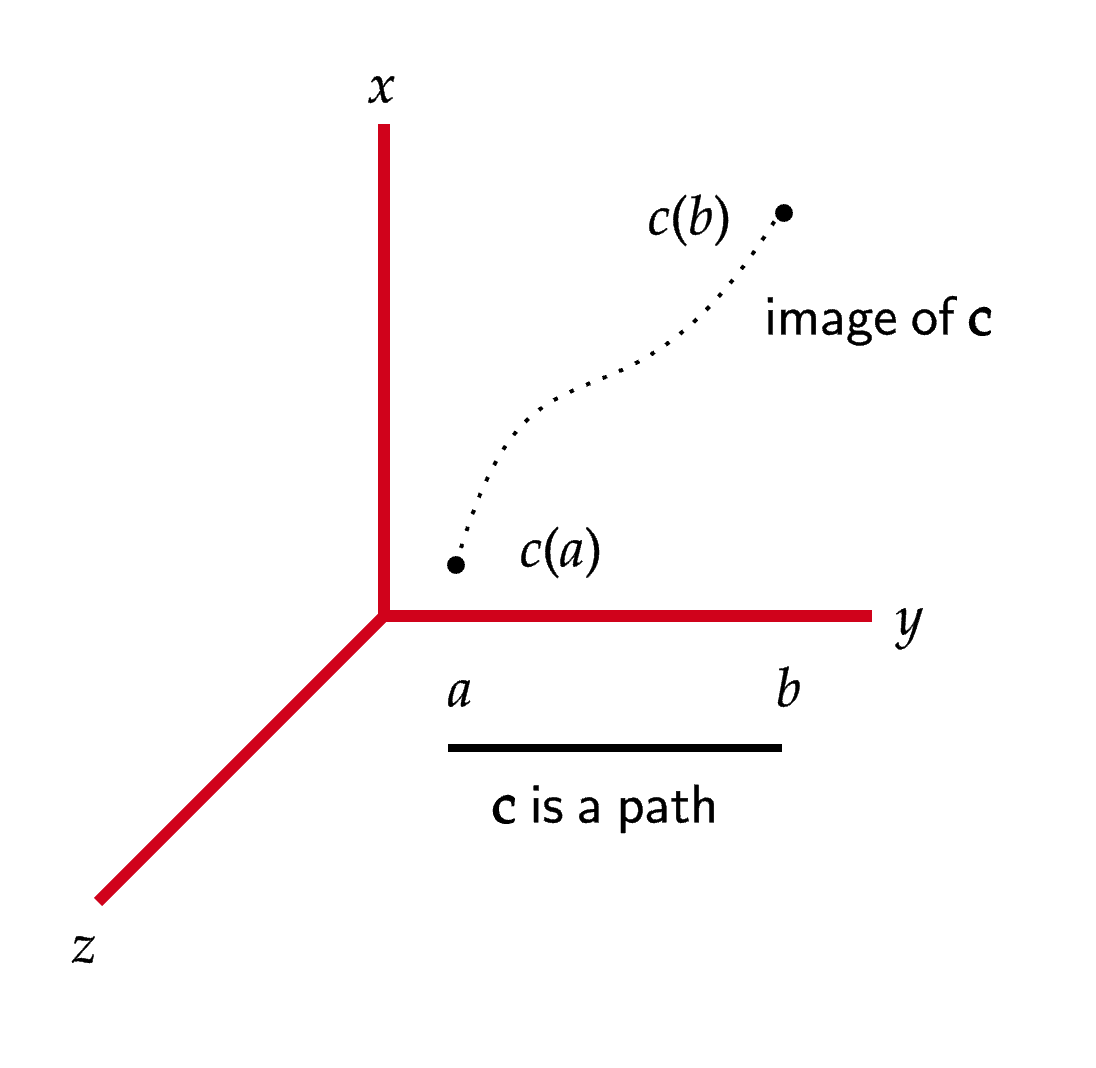
\includegraphics[width=0.8\textwidth]{figures/wk-2/fig-27.png}
\end{center}
\end{marginfigure}

\begin{ex}{Two Simple Curves}{label}
    Define two curves $\mathbf{c}_1$ and $\mathbf{c}_2$ on the interval $[0, 1]$ as follows,
    \begin{align*}
        &\mathbf{c_1}(t)=(t, t) \\
        &\mathbf{c_2}(t)=(2t, 2t) \\
    \end{align*}
    \begin{center}
    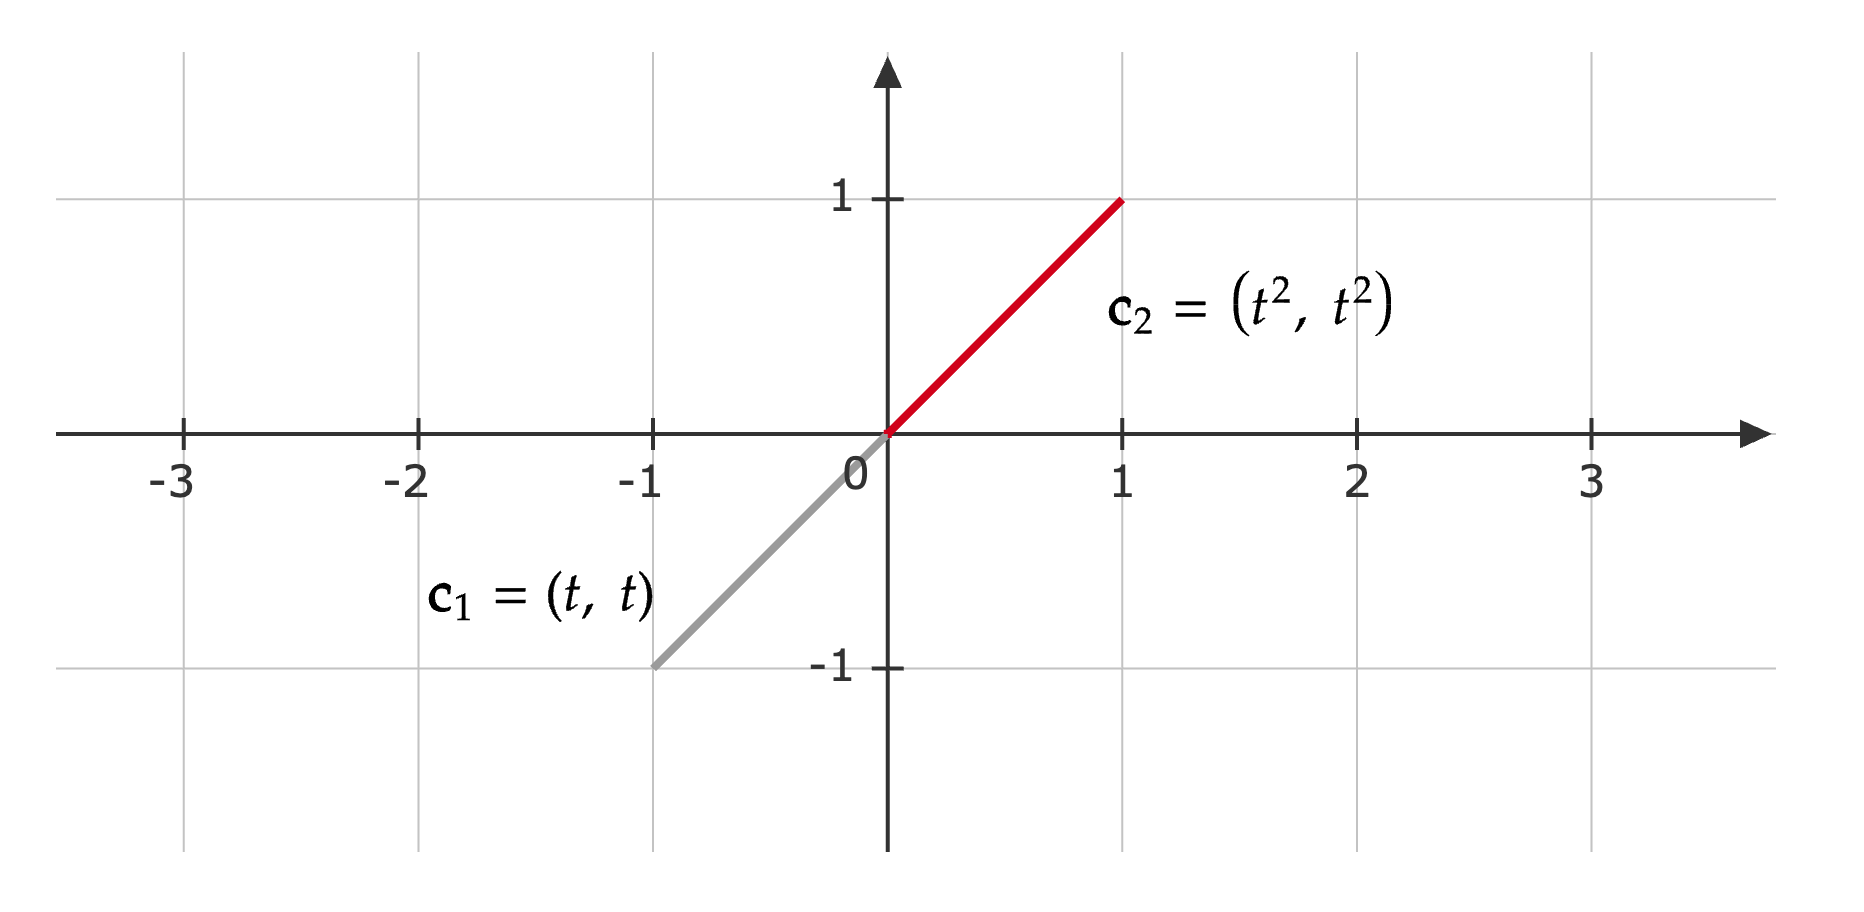
\includegraphics[width=0.8\textwidth]{figures/wk-2/fig-28.png}
    \end{center}
    Observe that $\mathbf{c}_1([0,1])=\mathbf{c}_2([0,1])$ but $\mathbf{c}^{\prime}_1(t) \neq \mathbf{c}^{\prime}_2(t)$,
    \[\mathbf{c}_1^{\prime}(t)=(1,1) \quad \quad \quad \mathbf{c}_2^{\prime}(t)=(2 t, 2 t)\]
    $\left\|\mathbf{c}_1(t)\right\|$ is constant, but $\left\|\mathbf{c}_1(t)\right\|$ is not.
    \begin{align*}
        &\left\|\mathbf{c}_1(t)\right\|=\|(1,1)\|=\sqrt{1^2+1^2}=\sqrt{2} \\
        &\left\|\mathbf{c}_2(t)\right\|=\sqrt{4 t^2+4 t^2}=2 \sqrt{2} t
    \end{align*}
\end{ex}

\begin{ex}{Unit Circle}{label}
    Define a curve $\mathbf{c}$ on the interval $[0, 2\pi]$ as follows,
    \begin{align*}
        &\mathbf{c}(t)=(\cos t, \sin t)
    \end{align*}
    The unit circle $\{(x, y) \mid x^2+y^2=1\}$ is parameterized by $\mathbf{c}$.
    \begin{center}
    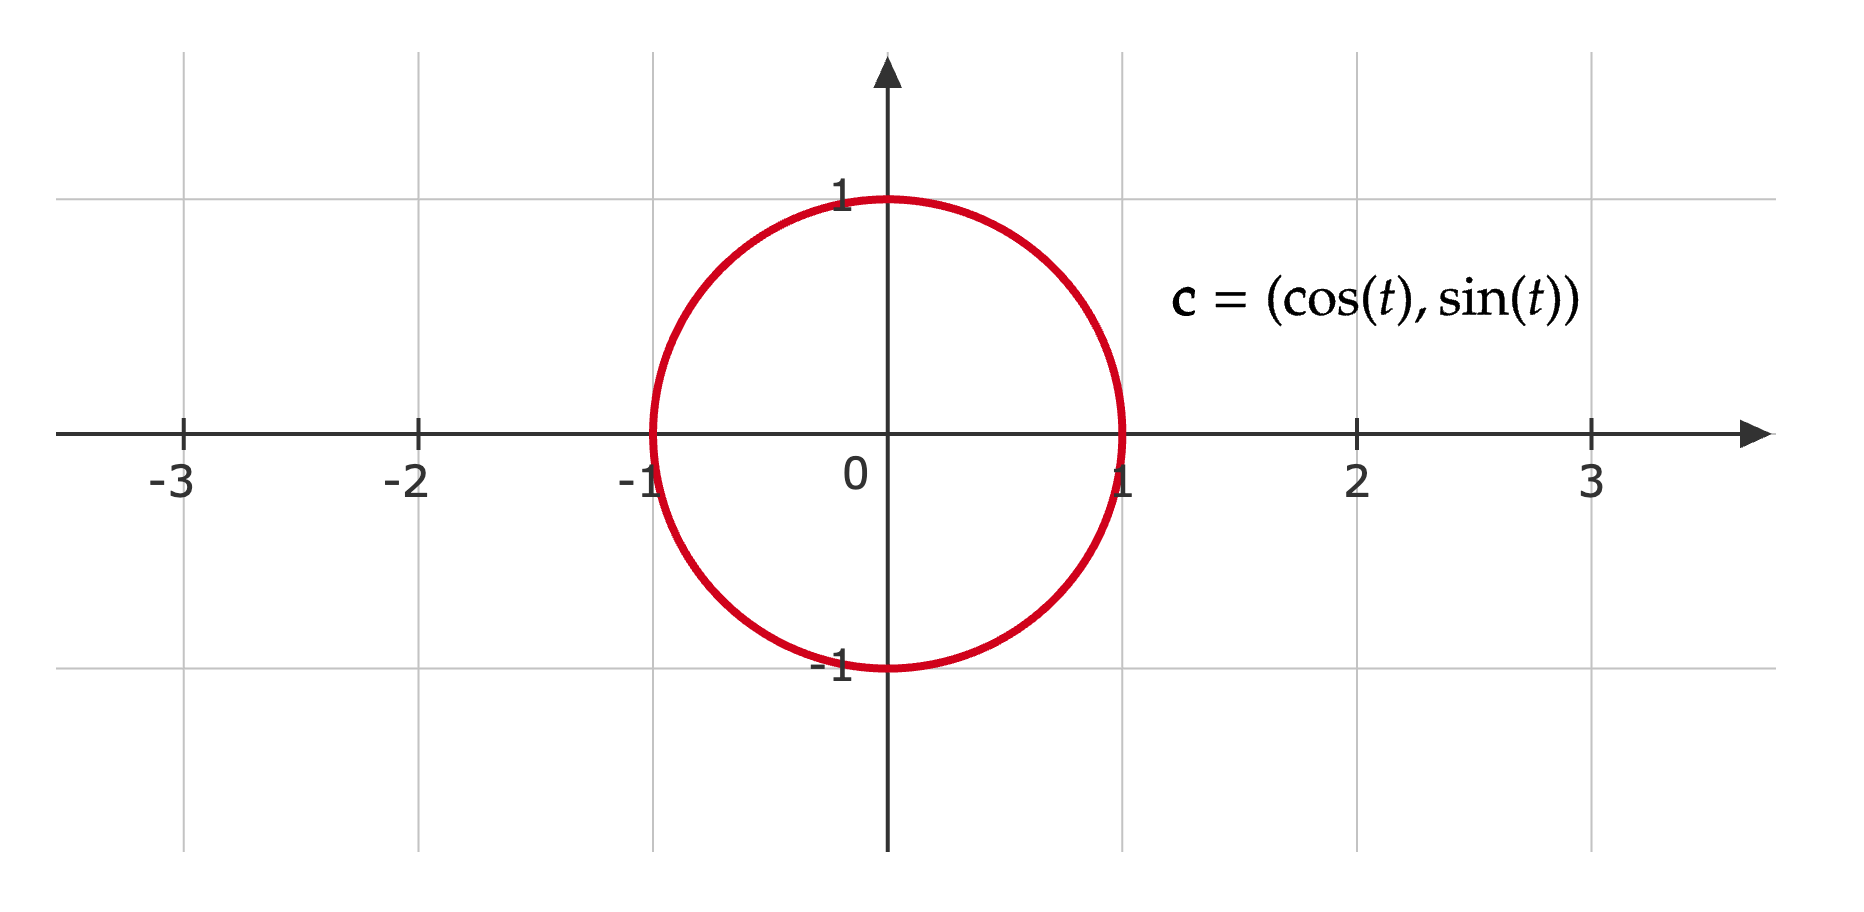
\includegraphics[width=0.8\textwidth]{figures/wk-2/fig-29.png}
    \end{center}
\end{ex}

\begin{thm}[Differentiation of Paths]
    If a path $\mathbf{c}$ with component functions $x_1(t), \cdots, x_n(t)$ is differentiable, then its derivative is
    \[z^{\prime}(t)=\left[\begin{array}{c}
    d x_1 / d t \\
    d x_2 / d t \\
    \vdots \\
    d x_n / d t
    \end{array}\right]\]
\end{thm}

\begin{prop}
    $\mathbf{c}^{\prime}(t)$ is the \textbf{tangent vector} at the point $\mathbf{c}(t)$.
\end{prop}

\begin{marginfigure}
    We can apply the typical differentiation rules to the components of $\mathbf{c}(t)$.
\end{marginfigure}

\subsection{Directional Derivatives}
\begin{defn}[Directional Derivative]
    Let $f: \R^3 \rightarrow \R$. The \textbf{directional derivative} of $f$ at $\mathbf{x}_0$ along the vector $\mathbf{v}$ is,
    \[\left(\nabla_{\mathbf{v}} f\right)\left(\mathbf{x}_0\right)=\left.\frac{d}{d t}\right|_{t=0} f\left(\mathbf{x}_0+t \mathbf{v}\right) = \lim _{h \rightarrow 0} \frac{1}{h}\left(f\left(\mathbf{x}_0+h \mathbf{v}\right)-f\left(\mathbf{x}_0\right)\right)\]
\end{defn}

\begin{rmk}
    Conventionally, we take $\mathbf{v}$ so that $\|\mathbf{v}\| = 1$.
\end{rmk}

\begin{ex}{Computing Rate of Change in a Direction}{label}
    We will compute the rate of change of
    \[f(x, y)=\left(x^2+y^2\right) \cdot e^{-\left(x^2+y^2+10\right)}\]
    at $(2,1)$ in the direction pointing towards $(0,0)$. To do this, we will find $\left(\mathbf{\nabla}_{\mathbf{v}} f\right)(2,1)$, where $\mathbf{v}$ is the unit vector pointing from $(2,1)$ towards $(0,0)$. We require the partial derivatives,
    \begin{align*}
        &f_x=2 x \cdot e^{-\left(x^2+y^2+10\right)}+\left(x^2+y^2\right) \cdot e^{-\left(x^2+y^2+10\right)}(-2 x) \\
        &f_y=2 y \cdot e^{-\left(x^2+y^2+10\right)}+\left(x^2+y^2\right) \cdot e^{-\left(x^2+y^2+10\right)}(-2 y)
    \end{align*}
    Evaluating $f_x$ and $f_y$ at $(2,1)$,
    \begin{align*}
    &f_x(2,1)=-16 e^{-15} \\
    &f_y(2,1)=-8 e^{-15}
    \end{align*}
    We obtain the final result,
    \[\left(\mathbf{\nabla}_{\mathbf{v}} f\right)(2,1)=\frac{256}{\sqrt{5}} \cdot e^{-15}\]
\end{ex}

\begin{thm}
    $\left(\mathbf{\nabla}_{\mathbf{v}} f\right)\left(\mathbf{x}_0\right)=\mathbf{v} \cdot(\mathbf{\nabla} f)\left(\mathbf{x}_0\right)$
\end{thm}

\begin{proof}
    Observe that,
    \begin{align*}
        \frac{d}{d t} f\left(\mathbf{x}_0+t \mathbf{v}\right) &=(\mathbf{\nabla} f)\left(\mathbf{x}_0+t \mathbf{v}\right) \cdot \frac{d}{d t}\left(\mathbf{x}_0+t \mathbf{v}\right) \\ &=(\mathbf{\nabla} f)\left(\mathbf{x}_0+t \mathbf{v}\right) \cdot \mathbf{v} 
    \end{align*}
    Plugging in $t = 0$,
    \[\left.\frac{d}{d t}\right|_{t=0} f\left(\mathbf{x}_0+t \mathbf{v}\right)=(\mathbf{\nabla} f)\left(\mathbf{x}_0\right) \cdot \mathbf{v}\]
\end{proof}

\begin{cor}
    If $\mathbf{x}_0 \in U$ is such that $(\mathbf{\nabla} f)\left(\mathbf{x}_0\right) \neq \mathbf{0}$, then $(\mathbf{\nabla} f)\left(\mathbf{x}_0\right)$ indicates the direction of steepest increase for $f$ at $\mathbf{x}_0$.
\end{cor}

\begin{proof}
    Using Theorem 7,
    \begin{align*}
        \left(\mathbf{\nabla}_{\mathbf{v}} f\right)\left(\mathbf{x}_0\right)
        &= \mathbf{v} \cdot (\mathbf{\nabla} f)\left(\mathbf{x}_0\right) \\
        &= \|\mathbf{v}\| \cdot \|(\mathbf{\nabla} f)\left(\mathbf{x}_0\right)\| \cos\theta \\
        &= \|(\mathbf{\nabla} f)\left(\mathbf{x}_0\right)\| \cos\theta \text{ since } \mathbf{v} \text{ is a unit vector}
    \end{align*}
    This expression is maximized when $\theta = 0$, which occurs when $\mathbf{v}$ and $(\mathbf{\nabla} f)\left(\mathbf{x}_0\right)$ are parallel. That is, when $\mathbf{v}$ points to $(\mathbf{\nabla} f)\left(\mathbf{x}_0\right)$.
\end{proof}

\begin{marginfigure}
    $(\mathbf{\nabla} f)\left(\mathbf{x}_0\right)$ indicates the direction of steepest increase for the function $f$.
    \begin{center}
    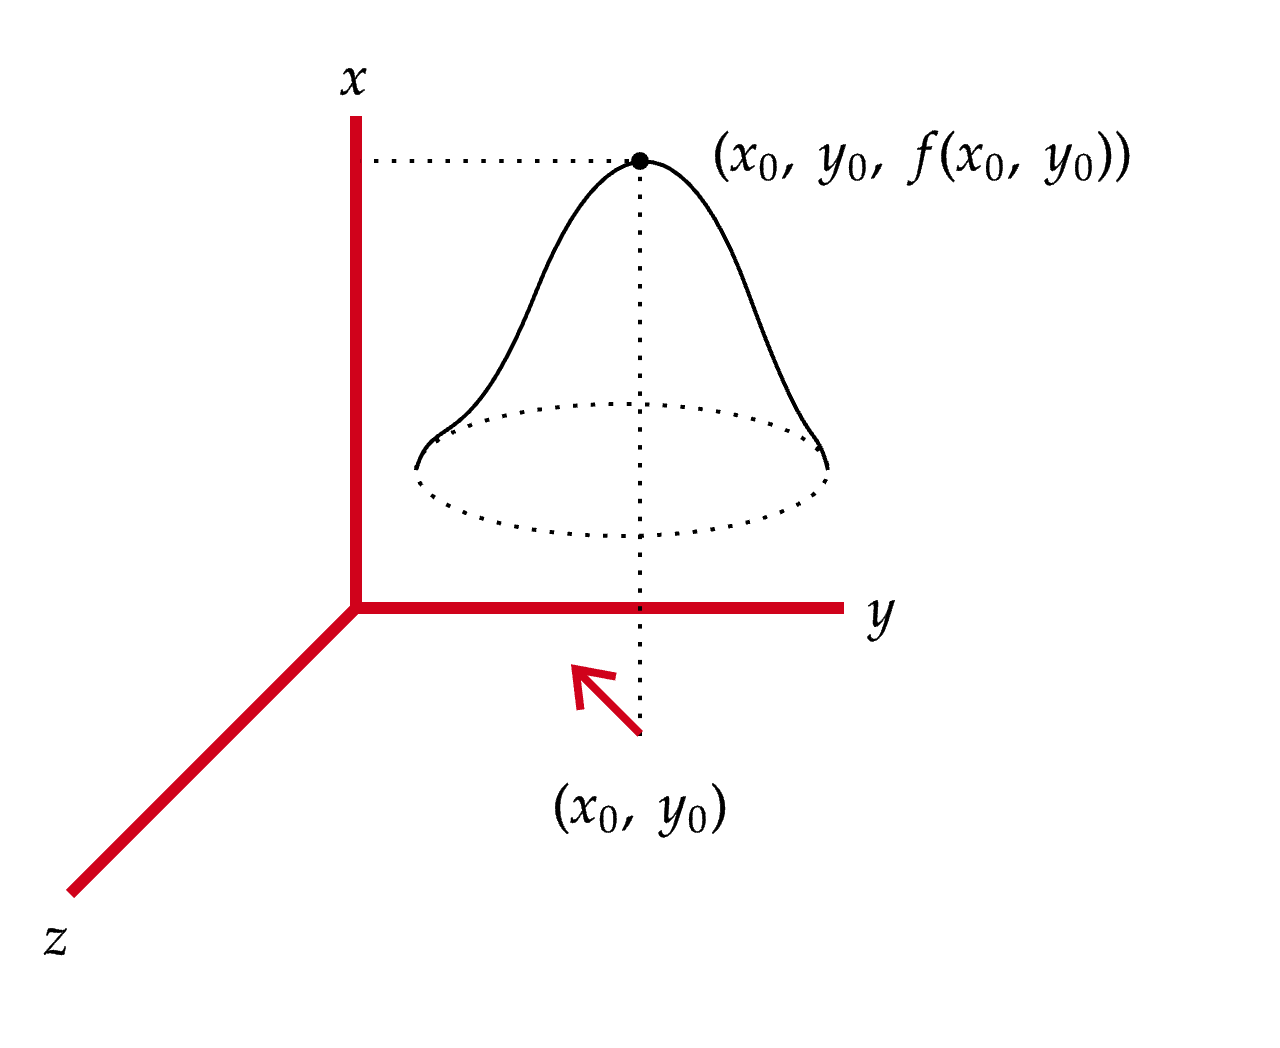
\includegraphics[width=\textwidth]{figures/wk-3/fig-30.png}
\end{center}
\end{marginfigure}

\begin{rmk}
    The gradient points in the direction in which the values of $f$ change most rapidly, whereas a level surface lies in the directions in which they do not change at all. Hence, for $f$ reasonably behaved, the gradient and the level surface will be perpendicular.
\end{rmk}

\begin{ex}{$f(x, y)=1-x^2-y^2$}{label}
    Consider the curve $f: \R^2 \rightarrow \R$ defined by
    \[f(x, y)=1-x^2-y^2\]
    The gradient of $f$ is given by,
    \[(\mathbf{\nabla} f)(\mathbf{x})=\left(-2 x -2 y\right)\]
    which at $(x_0, y_0, z_0) = \left(\frac{1}{\sqrt{3}}, \frac{1}{\sqrt{3}}, \frac{1}{3}\right)$ gives the tangent plane,
    \[z-\frac{1}{3} = -\frac{2}{\sqrt{3}}(x - \frac{1}{\sqrt{3}}) - \frac{2}{\sqrt{3}}(y-\frac{1}{\sqrt{3}})\]
\end{ex}